\documentclass{llncs}

\usepackage{graphicx}
%
\usepackage{geometry} % to change the page dimensions
\usepackage{multirow}
\usepackage{subfigure}


\geometry{a4paper}

\begin{document}


\title{Implementaci\'on de un Sistema Recuperaci\'on de Informaci\'on utilizando Redes Neuronales}

\author{Andy Gonz\'alez Pe\~na, Juan Eray \'Alvarez Hern\'andez}

\institute{MATCOM, Universidad de la Habana}
\maketitle


\begin{abstract}

Este trabajo recopila los puntos claves que conforman la implementaci\'on de un sistema de recuperaci\'on
de informaci\'on aunque no pretende proponer la mejor soluci\'on pero si una funcional para la aplicaci\'on
de los modelos de redes neuronales en la teor\'ia de los sistemas de recuperaci\'on de informaci\'on.

\end{abstract}

\section{Introducci\'on}\label{sec:Introduction}

Comenzaremos describiendo la estructura de la implementaci\'on, enumerando sus dependencias y definiendo la entrada y salida
del programa, con ello se va explicando su funcionamiento de manera general. \\
Luego para profundizar, subdividiremos las distintas tareas en cuatro  m\'odulos de los cuales se argumentan, de igual manera, su
funcionamiento y estructura demostrando el cumplimiento de los puntos requeridos en cada uno de ellos.\\
Finalmente, se enumeran ejemplos de acuerdo con los resultados obtenidos que muestran los puntos fuertes y d\'ebiles de la
implementaci\'on con el prop\'osito de darle continuidad al proceso de refinamiento en el que actualmente se encuentra.\\

\section{Estructura}\label{sec:Structure}

El proyecto se prefiere ver como un todo y aun as\'i consta de cuatro m\'odulos: interfaz de usuario, procesamiento de texto,
\'indice y modelado, todos implementados utilizando {\textit{Python}} (v3.6) con entradas y salidas sobre documentos de tipo
 {\textit{JSON}} que definen su comportamiento en cada instancia de la ejecuci\'on. \\
Cada m\'odulo existe en proceso diferente del sistema operativo y, \'unicamente, se relacionan mediante accesos al disco duro
para consultar los archivos de entrada y salida, para ello se cre\'o un sistema de notificaciones.\\
Todo fichero {\textit{JSON}}, como es conocido, son b\'asicamente diccionarios de llave-valor, entonces cada m\'odulo cuando
emita una salida escribir\'a la estampilla de tiempo que le corresponde logrando de esta forma que el m\'odulo que utilice ese
fichero como entrada sepa que ha ocurrido un cambio al mismo y sea capaz entonces de efectuar sus operaciones.\\
El orden de la comunicaci\'on es definido seg\'un su necesidad, en primera instancia se encuentra el m\'odulo de la interfaz de
usuario que emite como salida la propia entrada del m\'odulo de modelado y espera como entrada la salida del mismo. Mientras
los m\'odulos de procesamiento de textos e indizado se comportan de igual manera para la modelaci\'on no se comporta as\'i
como en un proceso plano, sino que se divide en tres instancias enviando y recibiendo de los otros m\'odulos hasta que logra
emitir la salida concisa que fue requerida por la interfaz de usuario. \\
En las secciones correspondientes a cada uno de ellos se discutir\'an los aspectos de su implementaci\'on y se definir\'an, de 
manera expl\'icita como se comportan para emitir una salida de datos consecuente a su situaci\'on.\\
Mientras, de manera general, se define la arquitectura del software seg\'un la interrelaci\'on existente presente en cada par
como indica siguiente figura.\\

{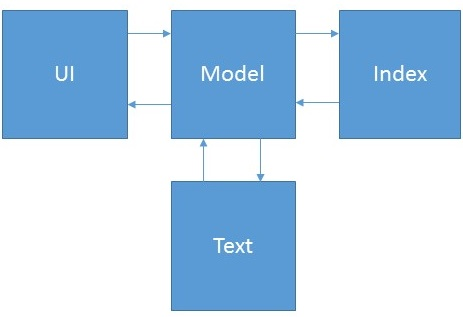
\includegraphics[]{structure}}
{\hfil\flushright{\textit{Fig 1. Estructura}}}

\subsection{M\'odulo Interfaz de Usuario}

Es una interfaz web minimalista que cumple con los est\'andares de dise\~no para el cual el usuario solamente podr\'a interactuar
seg\'un el sistema indique.

\subsubsection{Dependencias}

Creada en {\textit{Python}} utilizando {\textit{Flask}} como {\textit{framework}} en el que las plantillas renderizadas deber\'an ser
interpretadas debido al uso de cookies entonces se requiere de {\

\subsection{Perceptron}

%{\includegraphics[]{perceptron}}
%{\hfil\flushright{\textit{Fig 1. Perceptron}}}


Entre los primeros modelos aplicables de redes neuronales tenemos el \textit{perceptron}, el cual, en su visi\'on simplista, defin\'ia que
la funci\'on de activaci\'on neuronal, o actividad sin\'aptica, era una funci\'on lineal donde su entrada, de manera general, ser\'ian n\'umeros
reales y las salidas se daban en binario. En la figura 1 se muestra la analog\'ia de las tres neuronas del ejemplo de Hebb (y un $bias$).\\

Por definici\'on est\'a compuesto por dos capas de neuronas, una para la entrada y otra para la salida y se asumen completamente conectadas
entre s\'i, mientras que los costos o pesos de las conexiones para la entrada ya est\'an previamente fijados y luego a trav\'es de su algoritmo
interno de aprendizaje calcula los pesos para su salida. \\

%{\includegraphics[]{claseslineales}}
%{\hfil\flushright{\textit{Fig 2. Clases Lineales}}}

Un ejemplo de uso de \textit{perceptron} es el de reconocer puntos en el plano bidimensional $(x_1, x_2)$ donde existen dos posibles clases de soluciones,
las cuales son linealmente separables y, por ende, luego de n\'umero finito de corridas a trav\'es del perceptron, este asegura su convergencia. \\

Sin embargo, exactamente ese fue uno de los problemas encontrados por Minsky y \-Papert en 1969, cuando lanzan un art\'iculo demostrando las limitantes
del perceptron. Si las clases de soluci\'on no eran linealmente separables entonces el modelo jam\'as converger\'a.

\subsection{Backpropagation}

En consecuencia, para resolver la limitaci\'on de separabilidad lineal, surge el \textit{perceptron} multicapas (MLP) el cual es, en principio, lo mismo que su propuesta
anterior con la diferencia de que entre las capas de entrada y salida existen $n-$capas tal que juntas toman el nombre de capas ocultas.\\
Adem\'as, se pretende que las conexiones intermedias tengan el mayor n\'umero de conexiones posibles con el objetivo final de optimizar la respuesta, aunque
en la pr\'actica no siempre se pueda tomar de esa forma.\\

%{\includegraphics[]{mlp1}}
%{\hfil\flushright{\textit{Fig 3. MLP}}}

Sin embargo, este modelo no ser\'ia capaz de reutilizar el algoritmo original para el aprendizaje de un \textit{perceptron}, al menos no hasta que en 1975 se lanza el
algoritmo de \textit{backpropagation}. \\

Para su aplicaci\'on, las neuronas del MLP se consideran en un estado constante de entradas y salidas, con una funci\'on no lineal de activaci\'on. Mientras se
asume un error $E$ para un ciclo determinado, se puede aplicar la regla del gradiente descendiente para encontrar la conexi\'on \'optima entre los pesos $w_{i,j}$
con lo cual se asegura que luego de n\'umero finito de ciclos el error $E$ ser\'a suficientemente peque\~no.\\

Entonces, para un ciclo $t+1$ la variaci\'on del peso de un nodo $\Delta w_{i,j}$ se calcula de la siguiente manera: \\

$\Delta w_{i,j} (t + 1) = lrate * Err_{j} * o_j * (1 - o_j) * o_i$ \\

Donde $Err_j$ es el error entre el valor deseado en la salida $y_j$ y el valor $o_j$ producido por la neurona $j$, lo cual puede ser expresado como $Err_j = |y_j - o_j|$. \\

En cada ciclo (iteraci\'on, \'epoca) el algoritmo consta de dos fases:\\

1. Hacia adelante es cuando las entradas pasan a propagarse hasta llegar a las neuronas de salida y computar un respuesta. \\

2. Hacia atr\'as es cuando el error es calculado y no cumple con los requisitos de m\'inimo, entonces se propaga hacia los nodos intermedios provocando los cambios
de peso $\Delta w_{i,j}.$\\

Mientras el error se propaga de vuelta, el $Err_i$ para un nodo $i$ intermedio es calculado multiplicando todos los errores $Err_j$ de todas las neuronas $j$ adyacentes
a la neurona $i$ mediante su peso correspondiente $w_{i,j}$. El procedimiento se repite hasta que el error global sea suficientemente peque\~no. \\

\section{Modelo}

En todo sistema de recuperaci\'on de informaci\'on derivado de los modelos algebraicos cl\'asicos, los vectores de documentos son comparados con los vectores de consulta
para calcular su relevancia y por ende los t\'erminos de \'indices en documentos y consultas deber\'an ser comparados y pesados para computar tal relevancia. \\

%{\centering\includegraphics[]{mlp2}}
%{\hfil\flushright{\textit{Fig 4. Modelo MLP para la RI}}}

Una red neuronal es una representaci\'on simplificada del cerebro humano utilizando grafos, donde los nodos se comportan como neuronas y las aristas como las
conexiones sin\'apticas. En cada instante, un nodo es definido por su nivel de activaci\'on (funci\'on de su estado inicial y las se\~nales que recibe como par\'ametro).
Entonces, dependiendo de su nivel de activaci\'on, un nodo $A$ podr\'ia emitir una se\~nal a otro nodo adyacente $B$. La fuerza de la se\~nal en el nodo $B$
depende directamente del peso asociado a la arista que une los nodos $A$ y $B$.\\

En el proceso de hacia atr\'as descrito anteriormente, tales se\~nales tienen relaci\'on directa con el error y por ende, mientras pasan \'epocas de ejecuci\'on tales
se\~nales se debilitan.\\

Para los nodos de consulta son asignados un valor de activaci\'on inicial de 1 (m\'aximo), con los cuales pasan a la siguiente capa de nodos de la red neuronal y env\'ian
su se\~nal de activaci\'on a los nodos correspondientes atenuadas seg\'un la normalizaci\'on de los pesos de sus aristas $\overline{w}_{i,q}$.\\

$\overline{w}_{i, q}$ = $\frac{w_{i, q}}{\sqrt{\sum_{i < t}{w^2_{i, q}}}}$ \\

De la misma forma se calcular\'an los pesos para cada arista entre sus nodos correspondien\-tes de las distintas capas de la red neuronal en cuesti\'on. Finalmente,
cuando la se\~nal llega a un nodo documento $d_j$ su nivel de activaci\'on est\'a dado por: \\

$\sum_{i < t}{\overline{w}_{i, q}\overline{w}_{i, j}} = \frac{\sum_{i < t}{w_{i,q}w_{i,j}}}{\sqrt{\sum_{i < t}{w^2_{i, q}}} \* \sqrt{\sum_{i < t}{w^2_{i, j}}}}$ \\

El cual coincide exactamente con la f\'ormula de relevancia del modelo cl\'asico vectorial para la primera iteraci\'on de la red neuronal.\\

\subsection{Definici\'on Formal}

Una red neuronal es un cu\'adruplo \\$RN = <Q, D, F, R>$ donde: \\

$Q - $Conjunto de nodos de consulta donde todos tienen nivel de activaci\'on m\'axima y los pesos de las aristas correspondientes son las componentes del vector
asociado a la consulta.\\

$D - $Conjunto de nodos de documentos con funciones de entrada y salida de se\~nales en la cual los pesos de las aristas que les inciden son las componentes del
vector asociado a la salida de la red neuronal.\\

$F - $Como derivado del modelo vectorial se enmarca en la teor\'ia del \'Algebra Lineal de vectores y sus operaciones sobre un espacio $t-$dimensional y, adem\'as,
involucra la teor\'ia de grafos, estos dirigidos y ponderados como parte de la propia teor\'ia de redes neuronales.\\

$R -$Funci\'on de relevancia (ranking) enuncia\-da anteriormente y la misma que en el modelo vectorial.\\

Como definici\'on conjunta se puede definir como una funci\'on $F:\overline{x} \rightarrow R, F(x, \Theta)$ tal que $\Theta$ contiene los par\'ametros
que permiten realizar un mapeo del objeto de entrada $x$ y se devuelve otro objeto $y$.\\

\subsection{Comparaci\'on}

A continuaci\'on se presentan los principales aspectos que definen un sistema de recuperaci\'on puestos en comparaci\'on con el modelo de Redes Neuronales.\\

\subsubsection{Framework}
Booleano - Teor\'ia de Conjuntos y \'Algebra Booleana \\
Vectorial - Espacio t-dimensional y \'Algebra Lineal \\
Redes Neuronales - Teor\'ia de Grafos, Espacio t-dimensional y \'Algebra Lineal

\subsubsection{Pesos}
Booleano - \{0, 1\} \\
Vectorial - $w_{i,j}$ \\
Redes Neuronales - $\overline{w}_{i, j}$

\subsubsection{Consultas}
Booleano -  Expresiones Booleanas \\
Vectorial - Vectores de peso \\
Redes Neuronales - Nodos

\subsubsection{Documentos}
Booleano -  Vectores Binarios \\
Vectorial - Vectores de peso \\
Redes Neuronales - Nodos

\subsubsection{Similitud}
Booleano -  \{0,1\} \\
Vectorial - $\cos{\alpha}$ \\
Redes Neuronales - $\cos{\alpha}$

\subsubsection{Dependencia}
Booleano -  No \\
Vectorial - No \\
Redes Neuronales - Si

\subsubsection{Correspondencia Parcial}
Booleano -  No \\
Vectorial - Si \\
Redes Neuronales - Si

\subsubsection{Ranking}
Booleano -  No \\
Vectorial - Si \\
Redes Neuronales - Si

\section{Ejemplo}

Para entender el funcionamiento de las redes neuronales, se presenta a continuaci\'on un ejemplo ilustrativo de un red neuronal dedicada al
reconocimiento de vocales a partir de una imagen.\\

%{\includegraphics[]{example}}\\
%{\hfil\flushright{\textit{Fig 5. Ejemplo. Reconocimiento en una imagen}}}

Primeramente, el sistema debe conocer las muestras de cada vocal parametrizadas:\\

A: 01110100011000111111100011000110001 \\

E: 11111100001000011100100001000011111 \\

I: 11111001000010000100001000010011111 \\

O: 01110100011000110001100011000101110 \\

U: 10001100011000110001100011000101110 \\

Fijar como n\'umero de entradas de la red 35, puesto que son 35 los n\'umeros de la matriz resultante de $7x5$ resultante de la parametrizaci\'on
y como n\'umero de salidas 5 ya que esa es la cantidad de vocales.\\

Note que en una primera instancia no es necesaria una capa oculta, de manera emp\'irica se pueden ir a\~nadiendo capas con el objetivo de optimizar
resultados o simplemente disminuir el tiempo en ejecuci\'on antes de dar tales resultados. Adem\'as, se puede evitar el uso de neuronas auxiliares (bias)
y se utiliza como funci\'on de activaci\'on la sigmoidal (aunque pueden ser muchas otras). \\
Se fijan los valores iniciales de $lrate$, $M$, $E_{min}$ como marco de trabajo donde:\\
- $lrate$ puede tomar valores entre 0 y 1. Usualmente se les da un valor medio. \\
- $M$ puede tomar valores entre 0 y 1. Se utiliza para asegurar que el algoritmo no se caiga en ciclos en ninguno de los pasos\\
- $E_{min}$ se define como cota de ejecuci\'on y es usualmente un valor lo suficientemente peque\~no tal que el resultado se considere una respuesta aceptable.

\section{Conclusiones}

El alza de nuevas de tareas de recuperaci\'on de informaci\'on demanda replantear muchas de las m\'etricas que consideramos correctas para evaluar la relevancia
de un documento en un sistema dada una consulta y, a la vez, para otra situaci\'on ser totalmente lo contrario. Es, por ende, que los modelos de Redes Neuronales
deber\'an no solo evolucionar desde el punto de vista computacional, es decir, en cuanto a temas de optimizac\'ion, sino que debe ser acompa\~nado de numerosos
aspectos que interac\-t\'uan sobre ellos. \\
Est\'a reflejado que a lo largo del tiempo, estos modelos han demostrado cuantiosos resultados para muchas ramas de la ciencia, con lo cual su importancia existe
m\'as all\'a del plano te\'orico, estando presentes en casi cada acci\'on tecnol\'ogica que cada persona promedio realiza al menos una o dos veces al d\'ia y a\'un se
encuentra en constante evoluci\'on.


\begin{thebibliography}{1}

\bibitem{mir}
Baeza-Yates, R., Ribeiro-Neto, B.:
Modern Information Retrieval.
Addison-Wesley, 1999
Longman Publishing Co., Inc., Boston, MA, USA

\bibitem{foundations}
Kasabov, Nikola.:
Foundations of Neural Networks, Fuzzy Systems and Knowledge Engineering.
MIT Press, 2002, Cambridge, MA, USA

\bibitem{paper}
Wilkinson, R., Hingston, P.:
Using the cosine measure in a neural network for document retrieval. 1991.
In Proc of the ACM SIGIR Conference on Research and Development. Chicago, USA.

\bibitem{mitra}
Mitra, B., Craswell, N.:
An Introduction to Neural Information Retrieval. 2018.
Foundations and Trends in Information Retrieval, Cambridge, UK.

\bibitem{lectures}
Kenter, T., Borisov, A., Van Gysel, C., Dehghani, M., de Rijke, M., Azarbonyad, H.:
Lectures on Neural Networks for Information Retrieval.
WSDN2018, University of Amsterdam, Netherlands.

\bibitem{conferencias}
Valle Vidal, C.:
Lectures on Artificial Neural Networks. 2009.
Universidad T\'ecnica Federico Santa Mar\'ia, Santiago, Chile

\bibitem{tesis}
Lopez, D., Navas, G.:
Dise\~no y Construcci\'on de una red neuronal de prop\'osito general.
2007, Universidad T\'ecnica Salesiana, Quito, Ecuador.

\end{thebibliography}

\end{document}